\documentclass[tikz,border=2pt]{standalone}
\usepackage{amsmath}
\usepackage{pgfplots}
\pgfplotsset{compat=1.18}
\usetikzlibrary{arrows.meta}
\begin{document}
% f(x)=sqrt(|x|): the sublevel set at level alpha=1 is the interval [-alpha^2,alpha^2]=[-1,1] (convex), so f is quasi-convex;
% f is not convex: the chord from (0,0) to (1,1) has height 1/2 at x=1/2, below f(1/2)=1/sqrt(2)~0.707.
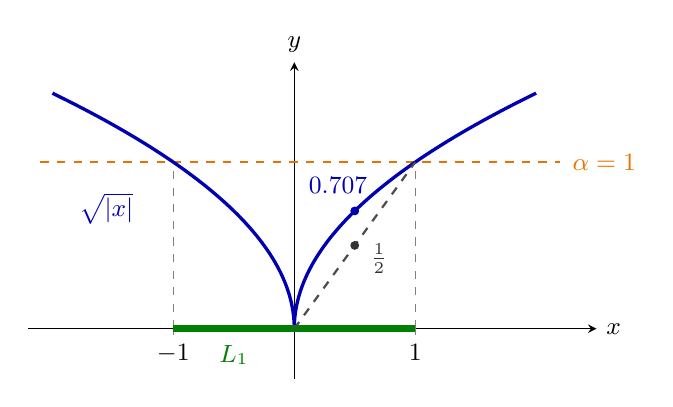
\begin{tikzpicture}[font=\small, >={Latex[length=2mm]}]
  \begin{axis}[
    axis lines=middle, xmin=-2.2, xmax=2.5, ymin=-0.3, ymax=1.6,
    xtick={-1,1}, ytick=\empty,
    xlabel={$x$}, ylabel={$y$},
    xlabel style={anchor=west}, ylabel style={anchor=south},
    width=8.8cm, height=5.6cm, clip=false
    ]
    \draw[orange!90!black, thick, dashed] (axis cs:-2.1,1) -- (axis cs:2.2,1);
    \node[orange!90!black, anchor=west] at (axis cs:2.22,1.0) {$\alpha=1$};
    \draw[gray, thin, dashed] (axis cs:-1,0) -- (axis cs:-1,1);
    \draw[gray, thin, dashed] (axis cs:1,0) -- (axis cs:1,1);
    \addplot[blue!70!black, very thick, domain=-1.4142:1.4142, samples=121, variable=\t] ({\t*abs(\t)},{abs(\t)});
    \node[blue!70!black, anchor=east] at (axis cs:-1.25,0.72) {$\sqrt{|x|}$};
    \draw[green!50!black, line width=2.4pt] (axis cs:-1,0) -- (axis cs:1,0);
    \node[green!50!black, anchor=north] at (axis cs:-0.5,-0.04) {$L_1$};
    \draw[gray!60!black, thick, dashed] (axis cs:0,0) -- (axis cs:1,1);
    \fill[gray!40!black] (axis cs:0.5,0.5) circle (1.6pt);
    \fill[blue!70!black] (axis cs:0.5,0.70711) circle (1.6pt);
    \node[blue!70!black, anchor=west] at (axis cs:0.04,0.86) {$0.707$};
    \node[gray!40!black, anchor=west] at (axis cs:0.55,0.42) {$\tfrac{1}{2}$};
  \end{axis}
\end{tikzpicture}
\end{document}
